
How do we benchmark the performance of quantum annealers and similar systems? How do we analyze our state of knowledge of that performance, if it is subject to a variety of nuisance parameters? How should we even define quantum speedup? In this dissertation, I will present work that I in collaboration with colleagues have done to answer these questions and apply those answers to a few test cases.

\section{Introduction}
As we look forward to the rapid development of new quantum computing devices with hundreds or thousands of qubits, particularly commercial devices and non-gate-based devices such as quantum annealers, we are faced with a
challenge. How does one ensure such devices really do what they claim, and aren't effectively classical? How does one evaluate the performance of such a device, what methods should one use to estimate performance on a given metric, and what metrics should one use? How do we do maintenance on the quantum state and ensure we can prevent or correct breakdowns and errors? These questions have to be settled before we can decide where to take our device on a test drive,
and what problems we should use our quantum computing devices to try to solve.

At this time, these new devices and plans for quantum annealing devices and various other quantum computing platforms are no longer the first of their kind. Several generations of programmable quantum annealers from D-Wave Systems have been made available to a small community of researchers, which has worked hard to answer the aforementioned questions. This community began largely groping in the dark, and has over the last five years answered many of the most basic questions, developing techniques to validate quantum annealers, methods to benchmark and estimate performance, and developing methods to suppress errors given the constraints of existing quantum annealers.

I have been fortunate to be members of the aforementioned community, which has given us an opportunity to work with the first several generations of quantum annealers, starting from the first commercially available such device, the $128$-qubit D-Wave One ``Rainier" processor, through two more generations of $512$ and $1152$ qubits, to the current $2048$-qubit D-Wave 2000Q processor.\footnote{A brief history: the Rainier processor ($108$ operational qubits) was the first to be installed at the USC-Lockheed Martin Quantum Computing Center at the USC Information Sciences Institute in 2011. Upgrades to the ``Vesuvius" ($504$ operational qubits) and ``Washington" ($1098$ operational qubits) processors followed in 2013 and 2016, respectively. Google installed ``Vesuvius" ($509$ operational qubits) and ``Washington" ($1097$ operational qubits) processors in the same years at NASA Ames. Los Alamos National Lab installed a ``Washington" processor ($1095$ operational qubits) in 2016. The 2000Q processor is now deploye at NASA Ames.} I have given significant thought to many of the aforementioned questions -- What is quantum speedup? How would we recognize it if it was there? Most importantly, how can we think rigorously about the state of our knowledge about the performance of a quantum annealer, particualrly when it is noisy or subject to a large space of nuisance parameters?

The discussion will draw mainly from the research I and colleagues have done on quantum annealers, and I apologize in advance to the many others who have contributed to this enterprise for not doing their work justice. I expect that some of the lessons learned will inform studies of future classes of quantum computing devices with many qubits.

My presentation of other's work aims to remain at a fairly high level, without giving a detailed technical account, for which I refer the reader to the original literature cited.

In this chapter \ref{ch:intro}, I will review some of the theory and literature of quantum annealing, describe some of the solvers that are often used to solve the Ising-type problems that existing annealers are meant to solve, and review some of the work on characterizing these systems. This chapter was heavily based on sections of my publications, particularly Ref \cite{job2018test}.

In chapter two \ref{ch:speedup}, I will present work on defining and detecting quantum speedup on a quantum annealer, and the initial application of that work toward benchmarking the D-Wave Two annealer using random Ising problems. This chapter was originally published as Ref \cite{speedup}.

In chapter three \ref{ch:benchmarking}, I will look in detail at the problem of estimating the performance of an algorithm (in particular a noisy quantum annealer). In particular, I'll discuss why one needs to think carefully about one's state of knowledge about the performance of an algorithm and how that differs from certain standard statistical techniques. That discussion also addresses some of the concerns with efficiency of benchmarking difficult problem classes, and proposes a mechanism to potentially significiantly reduce the computational effort of that task.

In chapter four \ref{ch:planted}, we'll again return to the application of some of the insights from chapters two and three, and give a partial solution to yet another problem in benchmarking -- how to compare algorithms on problems so difficult you cannot solve them via bruteforce. This is done through the introduction of planted solutions in Ising problems. We'll also address a theorem concerning the need to find an optimal annealing time for generic thermal or quantum annealing-type algorithms. This chapter was originally published as Ref \cite{Hen:2015rt}.

In chapter five \ref{ch:higgs}, we apply all these insights again to a very new context --- the use of quantum annealers in a machine learning context, namely binary classification. There we develop a model we call ``quantum annealing for machine learning'' or QAML and apply it to the problem of identifying Higgs boson decays in a sea of background events. This provides some additional motivation for considering how to benchmark algorithms where the algorithm in question is embedded into a complex analysis pipeline. This chapter was originally published as Ref \cite{myhiggs}.

Finally, in chapter six \ref{ch:conclusion}, we review all we've learned about the task of benchmarking and summarize a set of principles to guide future efforts. This chapter is a partly based on Ref \cite{job2018test}.

%%%%%%%%%%%%%%%%%%%%%%%%%%%%%%%%
\section{The Ising Hamiltonian and quantum annealing}
\label{app:algorithms}
%%%%%%%%%%%%%%%%%%%%%%%%%%%%%%%%
Consider the problem of finding the ground state of an Ising spin glass model described by a  ``problem Hamiltonian''
\begin{equation}
H_{\mathrm{Ising}} = -\sum_{i\in \mc{V}} h_i \sigma_i^z - \sum_{(i,j)\in \mc{E}} J_{ij} \sigma_i^z \sigma_j^z \ ,
\label{eq:H}
\end{equation}
with $N$ binary variables $\sigma_i^z = \pm 1$. The local fields $\{h_i\}$ and couplings $\{J_{ij}\}$ are fixed and define a {problem instance} of the Ising model.
 The spins occupy the vertices $\mc{V}$ of a graph $G=\{\mc{V},\mc{E}\}$ with edge set $\mc{E}$. For most of the work here, the graph is some variant of the Chimera graph, though chapter \ref{ch:higgs} includes work on fully connected Ising models. For an extremely broad ensemble of graphs, the Ising problem is NP-hard \cite{Barahona1982}.

\subsection{Quantum annealers}
Quantum annealers are envisioned as a way of solving (finding the ground state) of an Ising problem. To perform quantum annealing one maps the Ising variables $\sigma_i^z$ to Pauli $z$-matrices and adds a transverse magnetic field in the $x$-direction to induce quantum fluctuations, thus obtaining the time-dependent quantum Hamiltonian

\begin{equation}
\label{eq:Hquantum}
H(t) = -A(t) \sum_i \sigma_i^x +B(t) H_{\rm Ising}\ , \quad t\in[0,t_a]\ .
\end{equation}
The annealing schedule starts at time $t=0$ with just the transverse field term (i.e., $B(0)=0$) and $A(0)\gg k_B T$, where $T$ is the temperature, which is kept constant. The system is then in a simple quantum state with (to an excellent approximation) all spins aligned in the $x$ direction, corresponding to a uniform superposition over all $2^N$ computational basis states (products of eigenstates of the $\sigma_i^z$). During the annealing process the problem Hamiltonian magnitude $B(t)$ is increased and the transverse field $A(t)$ is decreased, ending with $A(t_a)=0$, and couplings much larger than the temperature: $B(t_a) \max(\max_{ij}|J_{ij}|,\max_i|h_i|) \gg k_BT$.
At this point the system will again be trapped in a local minimum, and by repeating the process one may hope to find the global minimum. Quantum annealing can be viewed as a finite-temperature variant of the adiabatic quantum algorithm \cite{farhi}, typically thought of as being restricted to classical final Hamiltonians, as above.

The D-Wave devices \cite{Harris2010,0953-2048-23-6-065004,berkley2010scalable,Johnson2011} are designed to be physical realizations of quantum annealing using superconducting flux qubits and programmable fields $\{h_i\}$ and couplings $\{J_{ij}\}$, and have connectivity matching the Chimera graph.

 The Chimera graph of a DW2X used in tests in chapter \ref{ch:higgs} is shown in Figure~\ref{fig:chimera_test-driving}, with it's annealing schedule in \ref{fig:schedule_test-driving}. The ideal Chimera graph is defined as follows. Each unit cell is a balanced $K_{4,4}$ bipartite graph. In the ideal Chimera graph the degree of each vertex is $6$. The left-hand side of each unit cell has connections to corresponding qubits in unit cells above and below, while the right-hand side has connections to corresponding qubits in cells to the left and right.A $N=8L^2$-vertex Chimera graph comprises an $L\times L$ grid of $K_{4,4}$ unit cells, and the (so-called {\sc TRIAD}) construction of Ref.~\cite{Choi2} can be used to embed the complete $4L+1$-vertex graph $K_{4L+1}$.
 The treewidth of such a graph is $4L+1 \sim \mc{O}(\sqrt{N})$ \cite{Choi2}. Dynamic programming can always find the true ground state of the corresponding Ising model in a time that is exponential in the treewidth, i.e., that scales as $\exp(a\sqrt{N})$.

 \begin{figure}[t]
  \centering
   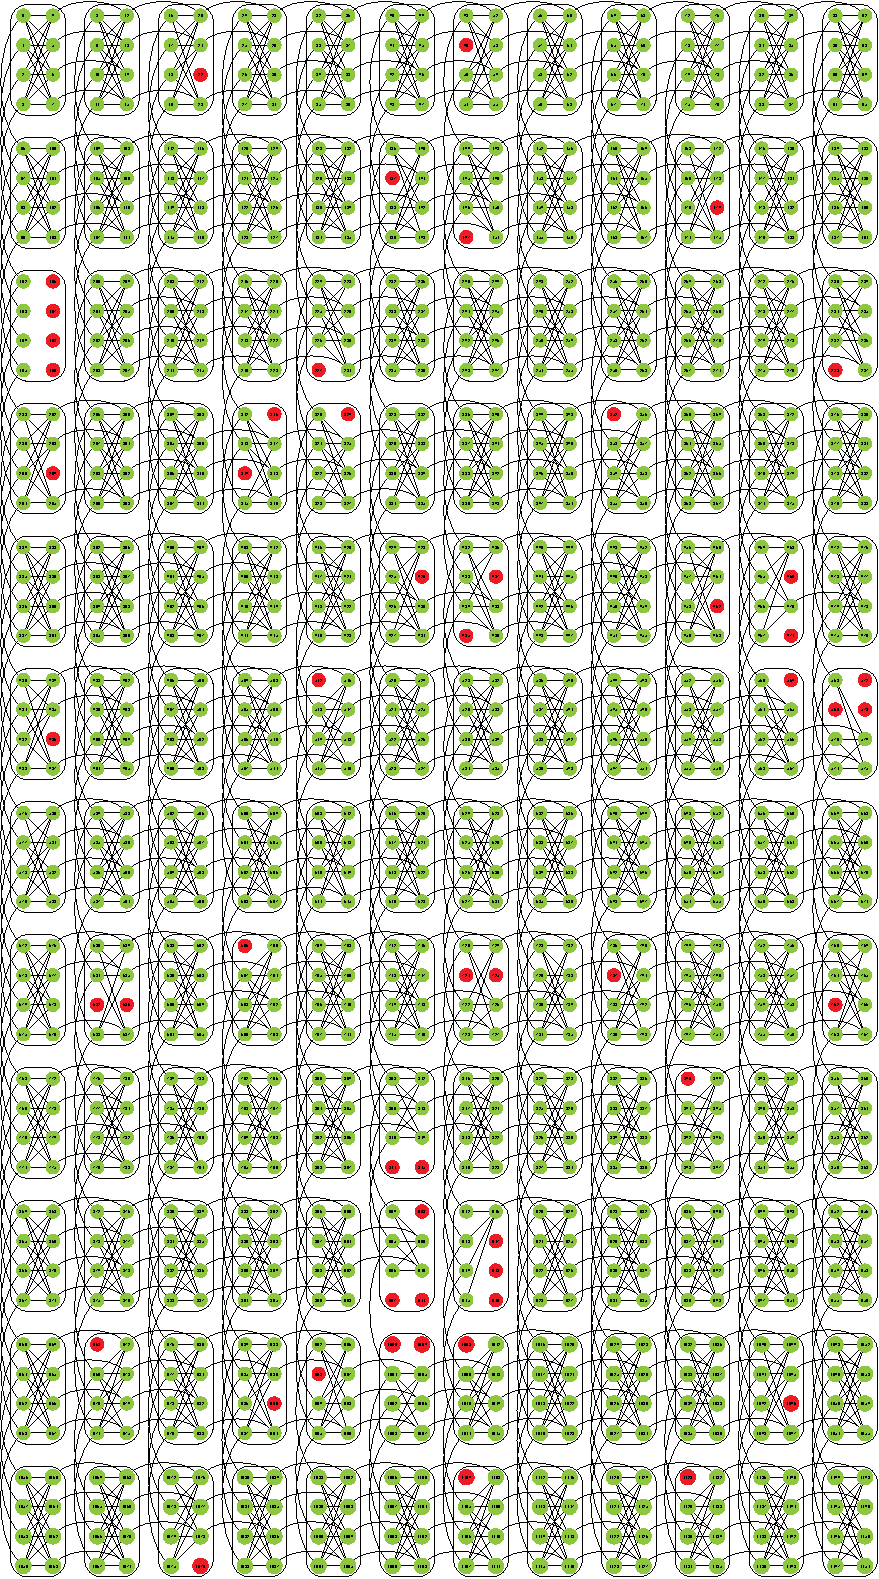
\includegraphics[width=.9\columnwidth]{chapters/Test-driving/chimera.pdf}
   \caption{An $1152$ qubit Chimera graph describing the D-Wave Two X processor at the University of Southern California's Information Sciences Institute. Inactive qubits are marked in red, active qubits ($1098$) are marked in green. Black lines denote active couplings (where $J_{ij}$ is programmable to be in the range $[-1,1]$) between qubits.}
   \label{fig:chimera_test-driving}
 \end{figure}

  \begin{figure}[t]
  \centering
   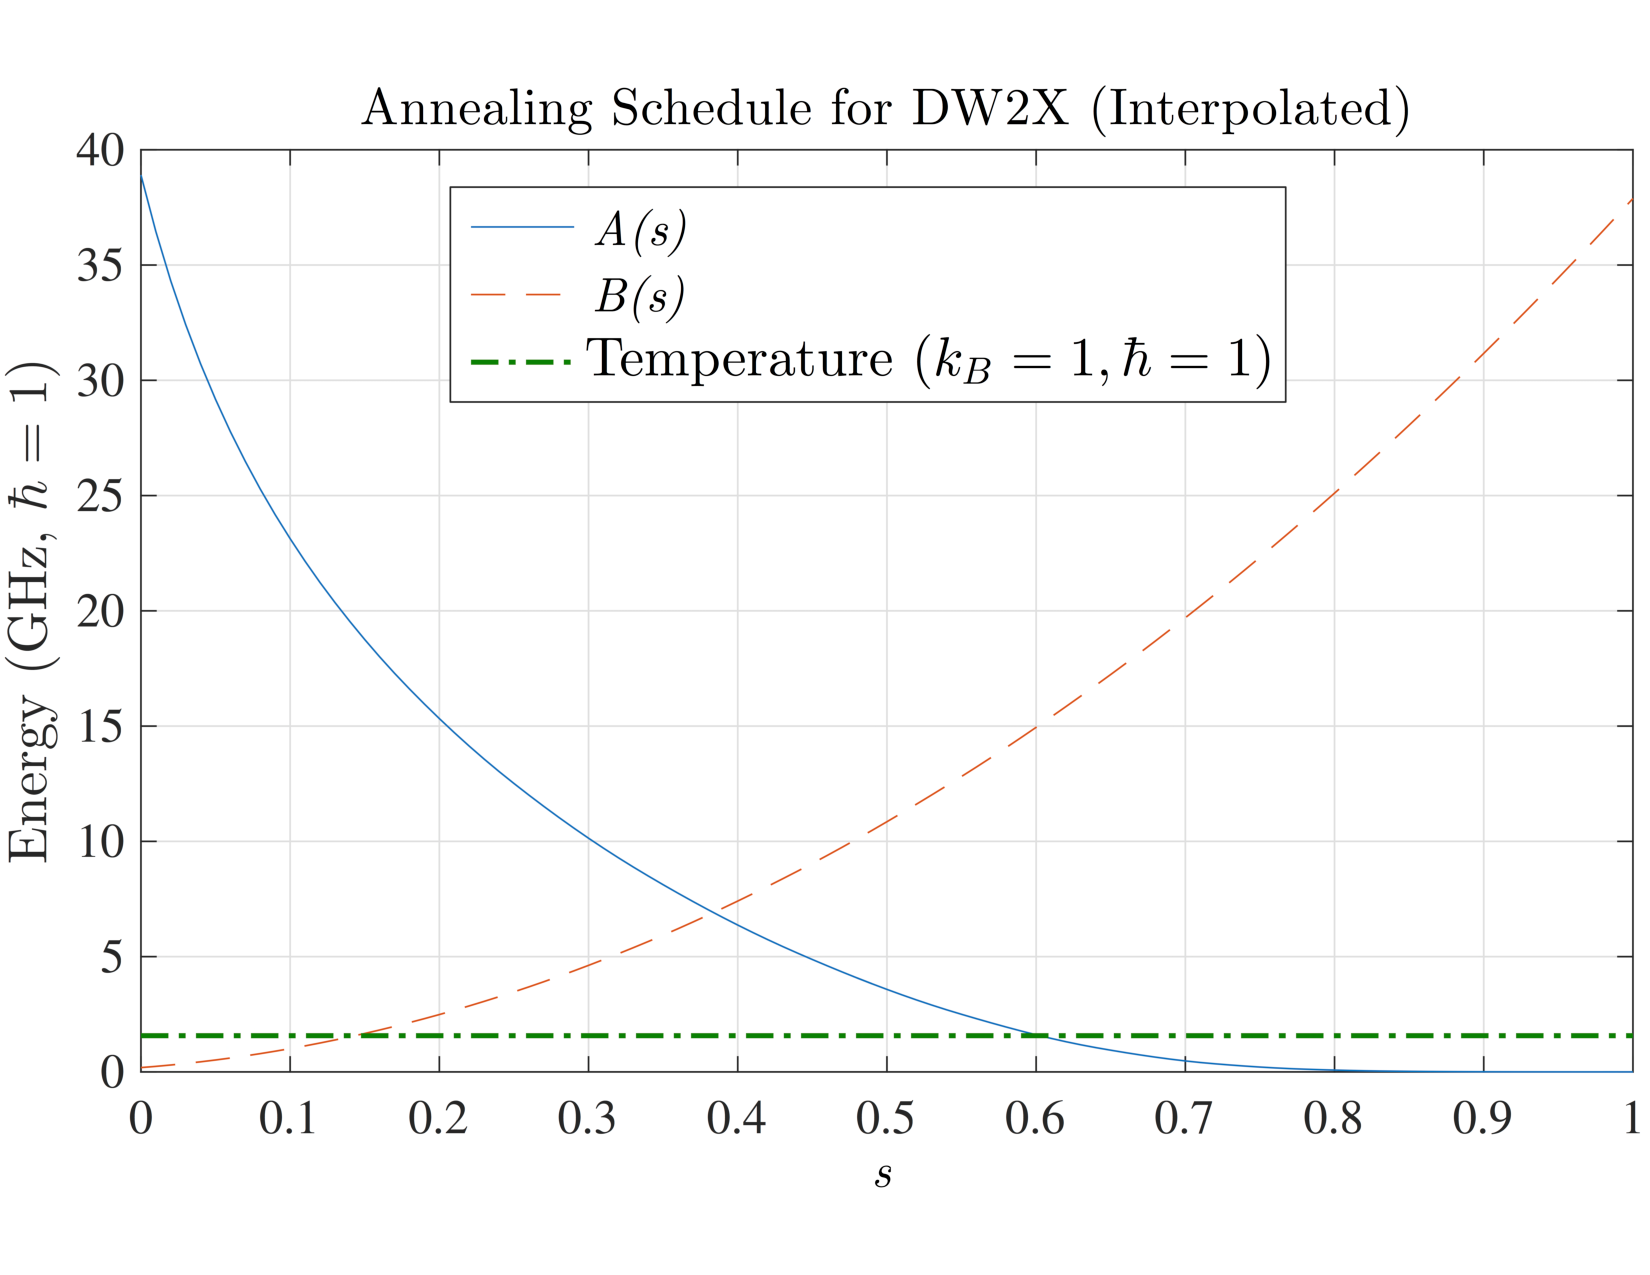
\includegraphics[width=0.9\columnwidth]{chapters/Test-driving/AnnealingSchedule.pdf}
   \caption{Annealing schedules for the D-Wave Two X processor described in Fig.~\ref{fig:chimera_test-driving}.}
   \label{fig:schedule_test-driving}
   \end{figure}

\section{Classical solvers}
The choice of classical solvers against which to compare the quantum device involves a few considerations. It is important to perform an apples-to-apples comparison, in that if the device is probabilistic, it would be misleading to measure its performance against a deterministic algorithm \cite{McGeoch,q108,MAX2SAT}. For a quantum annealer, a performance comparison to known heuristic algorithms for sampling low-energy states from Ising models is natural, such as SA \cite{kirkpatrick_optimization_1983,Isakov:2015ao}, parallel tempering (PT) \cite{Geyer:91,Earl:2005pd,katzgraber:06a}, and the Hamze-Freitas-Selby (HFS) algorithm (which searches all states on nodes that make up induces trees or small-treewidth subgraphs of the Ising model's connectivity graph) \cite{hamze:04,Selby:2014tx}. One might also compare to approximations of QA itself, in particular simulated quantum annealing (SQA) \cite{sqa1,Heim:2014jf,Crosson:2016fk}, or the SVMC algorithm \cite{SSSV}. All of these can be said to be ``solvers'' for the Ising problem on QA. But, to determine if the quantum device is truly useful in practice, it must also be compared to the \emph{best} algorithm for solving the \emph{original} (typically non-Ising problem) task. For example, when solving the graph isomorphism problem \cite{Zick:2015aa}, job-shop scheduling \cite{Venturelli:2015pi}, operational planning \cite{Rieffel:2015aa}, or portfolio optimization \cite{Rosenberg:2015}, the original problem must first be mapped into an Ising problem \cite{2013arXiv1302.5843L} and then embedded using the existing hardware connectivity graph \cite{Choi1,Choi2,klymko_adiabatic_2012}; the performance of the quantum device must be compared to the best algorithm for solving the original problem, and the mapping plus embedding steps can severely reduce performance. Note also that determining what the truly optimal classical algorithm is can be a daunting, or even impossible, challenge. In many cases one settles for an educated guess: the standard and/or currently best known algorithm(s). Finally, it is important to remember that any tests run on a quantum device that does not enjoy a fault tolerance guarantee cannot be reliably extrapolated to arbitrarily large sizes. I.e., in the absence of such a guarantee, a finite-size device provides evidence of what can be expected at larger sizes only provided that quantities such as the device temperature, coupling to the environment, and calibration and accuracy errors, can be appropriately scaled down. With this in mind, let us turn to a discussion of much of the benchmarking work done so far and some of the considerations that go into using large, noisy quantum devices.

\subsection{A brief description of some of the most relevant algorithms for solving Ising-type problems}

\subsubsection{HFS algorithm}
The HFS algorithm is due to Hamze \& Freitas \cite{hamze:04} and Selby \cite{Selby:2014tx}. This is a tree-based optimization algorithm, which exploits the sparsity and local connections of the Chimera (or other) graph to construct very wide induced trees and repeatedly optimizes over such trees until no more improvement is likely. It may also be used to sample from the marginal Gibbs state of each tree.

Let's briefly discuss the tree construction of the HFS algorithm.  It considers each part of the bipartite unit cell as a single $2^4$-dimensional vertex instead of four distinct $2$-dimensional vertices, resulting in a graph as depicted in Fig.~\ref{fig:SelbyTree}. The tree represented by the dark vertices covers $\approx 78\%$ of the graph, and such trees will cover $75\%$ of the graph in the limit of infinitely large Chimera graphs. Finding the minimum energy configuration of such a tree conditioned on the state of the rest of the graph can be done in $\mathcal{O} (N)$ time where $N$ is the number of vertices. Since the tree encodes so much of the graph, optimizing over such trees can quickly find a low-lying energy state. Since each sample takes a variable number of trees, we generally estimate time to solution as as the average number of trees multiplied by the number of operations per tree, with a time constant of $0.5\mu s$ per operation (derived from experiment).

More generally, one can also implement HFS in a graph-independent way, but building trees dynamically, however no studies in this work used this method.

\begin{figure}
\begin{center}
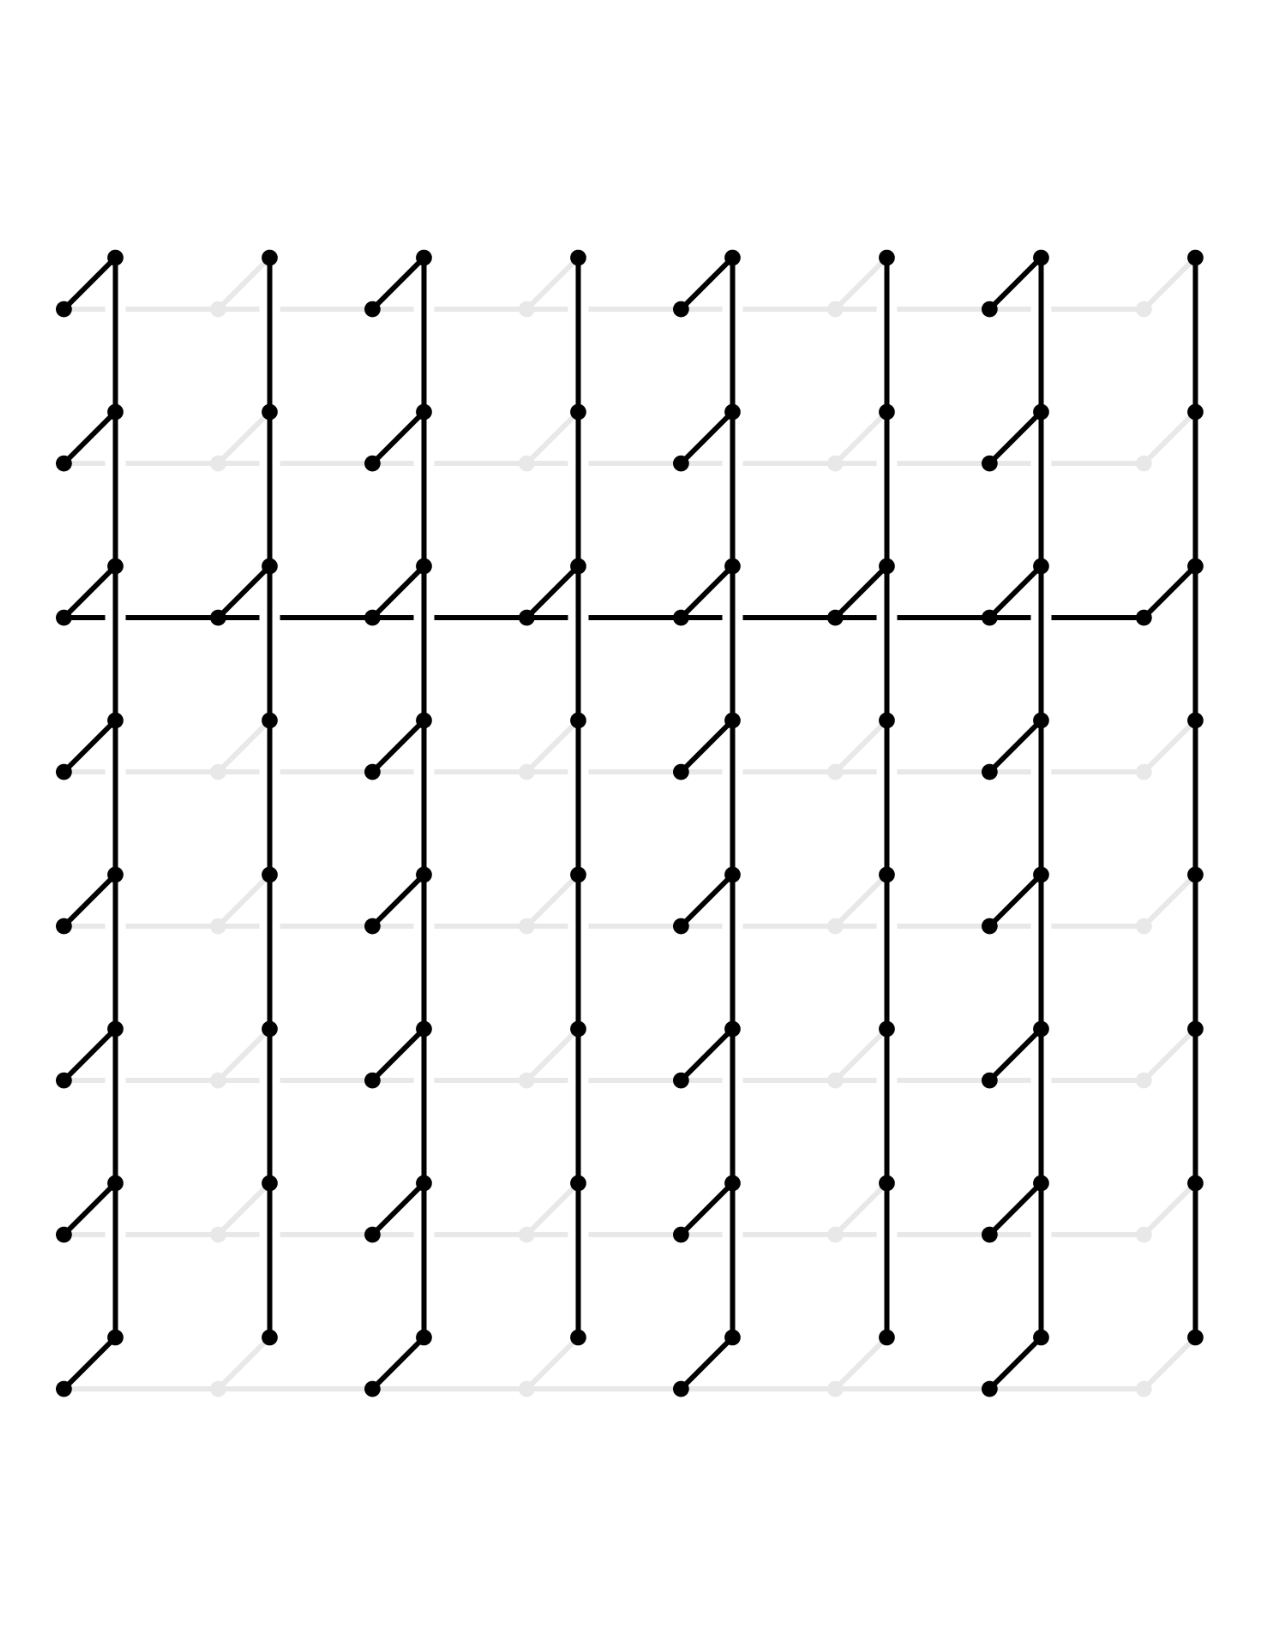
\includegraphics[width=\columnwidth]{chapters/Planted/selbytree}
\caption{An example of the view of the Chimera graph in the HFS algorithm. Each vertex is one half of a unit cell, and is $2^4$-dimensional. The algorithm repeatedly finds the minimum energy configuration of the graph over trees (like the one highlighted) given the state of the remaining vertices (in gray).}
\label{fig:SelbyTree}
\end{center}
\end{figure}


\subsubsection{Simulated Annealing}
The simulated annealing algorithm \cite{kirkpatrick_optimization_1983,Isakov:2015ao} typically uses a single spin-flip Metropolis update method.  In a single sweep, each spin is updated once according to the Metropolis rule: the spin is flipped, the change in energy $\Delta E$ is calculated.  If the energy is lowered, the flip is accepted, and if not, it is accepted with a probability given by the Metropolis probability:
%
\beq
P_{\mathrm{Met}} = \min \left( 1, \exp (- \beta \Delta E) \right)
\eeq
%
A linear annealing schedule in $\beta$ is typically used; Starting at $\beta_i = 0.01$, we increment $\beta$ in steps of  $\delta\beta = (\beta_f-\beta_i)/(S-1)$ where $S$ is the number of sweeps, up to $\beta_f$.

\subsubsection{Parallel Tempering}
Parallel tempering (PT) \cite{Geyer:91,Earl:2005pd,katzgraber:06a} is very similar to SA, except that one encodes many copies of the system at different temperatures, performing Monte Carlo update sweeps on each copy and then performing a swap between neighboring systems in temperature space with another Metropolis update. Choosing the ensemble of temperatures is relatively difficult, but there are heuristics which typically yield good results and are efficient \cite{katzgraber:06a}. Advanced versions with clever update mechanisms specifically tailored for Ising models, such as the isoenergetic cluster move discussed in Ref \cite{PhysRevLett.115.077201}, have proven to be exceptionally powerful. However, parallel tempering will receive no further attention here, as it was not used in any of the studies I've published.

\subsubsection{SSSV/SVMC}
The SSSV (Shin, Smith, Smolin \& Vazirani) or SVMC (spin-vector Monte Carlo) model was first proposed \cite{SSSV} as a classical model that reproduced the success probabilities of the DW1 device studied in Ref.~\cite{q108}, although there is growing evidence that this model fails to capture the behavior of the device for specific instances \cite{q-sig2,Albash:2014if,Boixo:2014yu}.  The model can be understood as describing coherent single qubits interacting incoherently by replacing qubits by O(2) rotors; the Hamiltonian can be generated by replacing $\sigma_i^x \mapsto \sin \theta_i$ and $\sigma^z_i \mapsto \cos \theta_i$.  The system is then ``evolved'' by Monte Carlo updates on the angles $\theta_i \in [0, \pi]$.  Although SSSV is not designed to be a fast solver, we studied it in chapter \ref{ch:planted} as a potential classical limit of the DW2 and checked what the scaling of such a classical limit would be.

\subsubsection{Simulated Quantum Annealing/Path Integral Monte Carlo}
SQA/PIMC \cite{sqa1,Heim:2014jf,Crosson:2016fk} is an annealing algorithm based on discrete-time path-integral quantum Monte Carlo simulations of the transverse field Ising model but using Monte Carlo dynamics instead of the open system evolution of a quantum system. This amounts to sampling the world line configurations of the quantum Hamiltonian \eqref{eq:Hquantum} while slowly changing the couplings. SQA has been shown to be consistent with the input/output behavior of the DW1 for random instances \cite{q108}, and we accordingly used a discrete-time quantum annealing algorithm.  Generally $64$ Trotter slices are used and an inverse temperature of $\beta=10$ (in dimensionless units, such that $\max(|J_{ij}|) = 1$) with linearly decreasing and increasing $A(t)$ and $B(t)$, respectively are used.  Cluster updates are performed only along the imaginary time direction.  A single sweep amounts to the following: for each space-like slice, a random spin along the imaginary time direction is picked.  The neighbors of this spin are added to the cluster (assuming they are parallel) according to the Wolff algorithm \cite{PhysRevLett.62.361} with probability $1 - e^{-2 J_{\perp}}$, where $J_\perp = -0.5 \ln \left[ \tanh A(t) \right]$ is the spin-spin coupling along the imaginary time direction.  When the cluster construction terminates, the cluster is flipped according to the Metropolis probability using the change in energy along the space-like direction associated with flipping the cluster.  Therefore a single sweep involves a single cluster update for each space-like slice.

\section{A quick review of quantum validation testing}
\label{sec:QVT}

Perhaps the first question one might ask when offered a quantum computational device is whether or not it is, in fact, quantum. In the case of quantum computational devices based on the circuit model and/or gates for quantum computing, the task of validation can be reduced to a Clauser-Horne-Shimony-Holt (CHSH) test between two parts of the device that are treated as black boxes \cite{Reichardt:2013db}. Alternatively, one may opt for quantum process tomography \cite{Chuang:97c,Mohseni:2008ly} or quantum gate set tomography \cite{blume2013robust,Greenbaum:2015aa}, wherein one applies many small computations and measures the results, verifying that they match the predictions of quantum theory. These predictions are available because the quantum computations in question typically involve few qubits and are thus readily implementable \cite{Childs:00,Blume-Kohout:2017aa}.

However, for other quantum computing paradigms, such as quantum annealing (QA) \cite{kadowaki_quantum_1998,RevModPhys.80.1061} and the broader field inspired by adiabatic quantum computing (AQC) \cite{farhi2001quantum,2002quant.ph.11152K,Kaminsky:2004fk,Albash-Lidar:RMP}, quantum tomography is not currently available for validation. This is for a variety of reasons. The key difference is that gate-based computations are modular: they can be broken into discrete time-local and space-local operations, operating effectively on only one or two qubits at a time, with the others left essentially unaffected, so the only requirement to validate even a long chain of computations is to validate those one- and two-qubit operations on individual qubits and pairs of qubits. For AQC-like platforms, the quantum computation is composed of a continuously time-varying Hamiltonian with many computational operators acting on the system at the same time. They are non-modular in the sense that they cannot be easily broken down into discrete chunks which can be validated separately. Future versions of such platforms may be more flexible and allow for approaches such as quantum tomography, but will still be unable to validate arbitrarily large computations due to the aforementioned nonmodularity of the computation. Meanwhile, partial alternatives such as tunneling spectroscopy have already been explored \cite{Berkley:2013bf}. Of course, in the absence of error correction and fault tolerance neither the gate model nor AQC are guaranteed successful validation.

Nevertheless, certain lessons can be ported over to non-gate-based approaches. One should, as in the circuit model, focus on small problems, with a small number of qubits, and one may hope that by studying such problems applied to many such overlapping sets that one can at least partially validate the operation of the device. From here, two paths for validation become available, depending on whether one can ``open the black box'' and perform measurements during the anneal or use measurements beyond what may be considered ``native'' to the device, or whether one is only able to use the device's output at the end of complete runs for testing.

\subsection{Types of validation: proof of quantumness, quantum supremacy, speedup-inferred quantumness, and classical model rejection}
In validating quantum annealers, one seeks to create an assignment to the $h$'s and $J$'s such that one can take some measurements which will conclusively demonstrate, for instance, quantum entanglement, in what might be called an experimental ``\emph{proof of quantumness}''.

A somewhat weaker and indirect type of validation is provided by ``\emph{quantum supremacy}" experiments \cite{Preskill:2012aa},
since they have the potential for complexity theoretic guarantees.\footnote{The term ``supremacy" has generated considerable controversy \cite{Qsupremacy-debate}. While we would prefer the adoption of an alternative such as ``hegemony" or ``supremeness", we recognize that ``supremacy" is likely here to stay due to its current widespread usage.}
 More specifically, quantum supremacy is a scenario where (part of) the polynomial hierarchy of complexity theory collapses if the quantum result could be replicated classically without slowdown \cite{Aaronson:2016aa,Bremner:2016aa,FarhiHarrow-QAOA,Gao:2017aa,Boixo:2016aa,Fefferman:2017ab}. While weaker than a direct proof of quantumness, a demonstration of quantum supremacy would be considered strong evidence for quantum computational power of a device, which may be considered inherently more interesting than a direct demonstration of, e.g., entanglement.

``\emph{Speedup-inferred quantumness}" is a related type of indirect validation based on a demonstration of quantum speedup \cite{speedup}\ref{ch:speedup} over the best classical solvers known for a task, which is often considered the holy grail of quantum information processing. Unlike quantum supremacy tests, speedup-inferred quantumness tests do not have complexity theoretic guarantees (an example in the circuit model would be Shor's algorithm \cite{Shor:97}). It appears that an unqualified quantum speedup would necessarily have to invoke quantum properties, and this might happen even if these properties remain poorly understood or characterized. Thus a certificate of quantumness might be assigned even in the absence of a direct demonstration of quantum properties such as entanglement. It should be recognized that this carries a certain element of risk. For example, suppose a new \emph{classical} optimization is discovered that outperforms all other classical and quantum optimization algorithms known to date (this is in fact what happened recently in a tug-of-war between quantum and classical optimization for the Max E3LIN2 problem \cite{Farhi:2014aa}). This algorithm could be deceptively marketed as a quantum algorithm providing speedup-inferred quantumness by a shrewd company claiming to own quantum computers, that provides black-box access only to run the new optimization algorithm. Thus any claim of speedup-inferred quantumness should always be treated with a healthy degree of skepticism as related to its quantum underpinnings, until actual evidence of quantum effects driving the algorithm is presented.

If none of prior three types (proof of quantumness, quantum supremacy, speedup-inferred quantumness) of validation are attainable, one may alternatively seek to show that on sufficiently small scale problems the results are only readily reproducible using a truly quantum model of the device, and cannot be replicated qualitatively using any existing classical model, in what might be called ``\emph{classical model rejection}''. This type of validation experiment does not provide a certificate of quantumness, since one can always invent a new and better classical model. Instead, one can only hope to exclude all ``physically reasonable'' classical models for the device. Moreover, classical model rejection can only be performed as long as it is feasible to carry out quantum model simulations, which limits system sizes to about $20$ qubits for master equation type models, using the quantum trajectories method \cite{Yip:2017}. Extrapolations to larger sizes are, as always, risky in the absence of fault tolerance guarantees.

One caveat regarding ``proof of quantumness" experiments is noteworthy. While demonstrations of entanglement can be considered ``proof of quantumness", they often require additional physical resources and measurement possibilities beyond those that may natively be embedded in a (commercial) quantum computational device or that are strictly required to implement the core algorithm, and thus may be impossible on certain platforms. Additionally, in practice, certain assumptions may be made in a ``proof of quantumness'' experiment which, when relaxed, render it effectively a ``classical model rejection'' experiment; we shall shortly see an example of this with the D-Wave quantum annealers.


\subsection{Experimental implementations of quantum validation tests}
\label{sec:QVT-expt}

The primary ``proof of quantumness'' experiment for quantum annealers was performed in Ref.~\cite{DWave-entanglement}, using an entanglement test on the D-Wave Two (DW2) generation of processors. Briefly, the work used quantum tunneling spectroscopy \cite{Berkley:2013bf} to estimate the populations of the first and second excited states of a combined probe-system Hamiltonian. They also measured the energy spectrum and found it to be consistent with the Hamiltonian the device was designed to implement, which provided a justification for the assumption that the measured populations were those of the energy eigenstates of the Hamiltonian.
This allowed for a reconstruction of the density matrix under the assumption that it is diagonal in the energy eigenbasis, enabling a computation of the negativity \cite{Vidal:02a} for all possible bipartitions of the system, the geometric mean of which was taken as a measure of the entanglement of the system. As it was found to be nonzero, the system is entangled. Further, by exploiting the theory of entanglement witnesses~\cite{Spedalieri:2012fk},
Ref.~\cite{DWave-entanglement} was able to show that even if the diagonality assumption is relaxed, the entanglement remains. This was used to conclude that the DW2 system tested displays entanglement at least on the scale of a single $8$-qubit unit cell.

It was noted in Ref.~\cite{Albash:2015pd} that these tests depended on the assumption that the device was well-described by Eq.~\eqref{eq:H} for an appropriate (programmed) choice of local fields and couplers for which the ground state is entangled, and that this assumption is not directly demonstrable by the experiments in \cite{DWave-entanglement}. Without that assumption, one must revert to a ``classical model rejection'' experiment in which one compares results of direct quantum simulations of the device and available classical alternatives to demonstrate that only the quantum model is consistent with the experimental observations. Ref.~\cite{Albash:2015pd} provides a detailed description of the experiments, but for our purposes the key takeaway is that only the quantum adiabatic master equation \cite{aqcME} can reproduce the output distribution from experiments, validating the approach in Ref.~\cite{DWave-entanglement}.

\begin{figure}[t]
\centering
 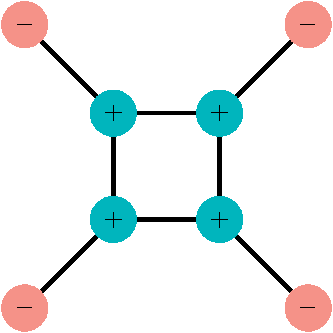
\includegraphics[height=1.75in]{chapters/Test-driving/signature}
\caption{The eight-spin Ising quantum signature Hamiltonian introduced in Ref.~\cite{q-sig}. The inner ``core" spins (green circles) have local fields $h_i = +1$ while the outer spins (red circles) have $h_i = -1$.  All  couplings are ferromagnetic: $J_{ij} = 1$ (black lines).}
\label{fig:signaturehamiltonian}
\end{figure}

Another branch of validation experiments of the classical model rejection type are the so-called ``quantum signature'' Hamiltonians and the consistency tests derived therefrom, introduced in Ref.~\cite{q-sig}, critiqued in Ref.~\cite{Smolin}, and further explored in Refs.~\cite{comment-SS,q-sig2,SSSV-comment}. Unlike the aforementioned entanglement tests, these experiments do not require access to the system during the annealing process, and are appropriate for cases in which the quantum device is a ``black box'' in which one can only control the inputs and measure the outputs. An example of a quantum signature Hamiltonian is shown in Fig.~\ref{fig:signaturehamiltonian}. These Hamiltonians take the form of a ring of tightly bound qubits each connected to a single outer qubit. The resulting Hamiltonian has the property that there is a large ($2^{N/2}$-dimensional) degenerate subspace of ground state configurations corresponding to arbitrary assignments to the outer qubits where all qubits in the inner ring are in the state $0$ (forming a ``cluster" connected by single spin flips applied to the outer ring). There is one additional ground state corresponding to flipping all the inner qubits to the state $1$, dubbed the ``isolated" state, since for a signature Hamiltonian with $2N$ qubits it is at least $N$ spin flips away from all other ground states. Thermal algorithms such as classical simulated annealing (SA) \cite{kirkpatrick_optimization_1983} will be weighted toward the isolated state, such that it will have the highest probability of occurrence of any ground state configuration, whereas an adiabatic quantum evolution will find the isolated state to be suppressed relative to the cluster states. Extensive simulations and experiments on a $108$ qubit D-Wave One (DW1) ``Rainier" processor matched qualitatively with the adiabatic master equation across all the parameters and statistics of the output distributions tested, though noise due to cross-talk made it very difficult to find quantitative agreement; at the same time all existing classical models failed to qualitatively match the DW1 in at least one of the tests \cite{q-sig2}.

A different approach to classical model rejection was taken in Ref.~\cite{q108}, which used random $J_{ij}=\pm 1$ instances of the Ising Hamiltonian in Eq.~\eqref{eq:H} to test the hypothesis that quantum annealing correlates well with two classical models: SA and classical spin dynamics \cite{Smolin} (also known as the Landau-Lifshitz-Gilbert model). The hypothesis was tested using the same DW1 processor. This work showed that these two classical models failed to correlate with the results for the distribution of ground state probabilities generated by the DW1 device, while the DW1 correlated very well with simulated quantum annealing (SQA), implemented using quantum Monte Carlo \cite{sqa1}. This was taken as evidence for quantum annealing on the scale of more than $100$ qubits, thus generalizing the conclusion of the earlier result \cite{q-sig} based on the $8$-qubit ``gadget" shown in Fig.~\ref{fig:signaturehamiltonian}. Shortly thereafter a new semiclassical Spin-Vector Monte Carlo (SVMC) model was introduced, also known as SSSV, the author initials of Ref.~\cite{SSSV}.\footnote{Both the spin-dynamics and SVMC models can be derived in a strong coupling limit from the anisotropic Langevin equation, starting from Keldysh field theory \cite{Crowley:2016aa}.}
In this model spins are treated as $O(2)$ rotors (effectively as single qubits), evolved according to the annealing schedule given in Eq.~\eqref{eq:Hquantum}, with Monte Carlo angle updates. The SVMC model correlated well with both the DW1 and SQA data, suggesting that although the DW1 device's performance is consistent with quantum annealing, it operated in a temperature regime where, for most random Ising spin glass instances, a quantum annealer may have an effective semi-classical description. This conclusion was challenged in Ref.~\cite{Albash:2014if}, which considered the excited state distribution rather than just the ground state distribution over random $J_{ij}=\pm 1$ Ising instances, as well as the ground state degeneracy. This work presented evidence that for these new measures neither SQA nor SVMC, which are classically efficient algorithms, correlated well with the DW1 experiments. The close correlation SQA and the SVMC model was explained by showing that the SVMC model represents a semiclassical limit of the spin-coherent states path integral, which forms the foundation for the derivation of the SQA algorithm.

The intense debate that arose around the original classical model rejection tests presented in Refs.~\cite{q-sig,q108}, in particular the critique presented in Refs.~\cite{Smolin,SSSV}, illustrates the risks associated with such tests---risks that materialize whenever a sufficiently clever new classical model is found that agrees with (some of) the data---as well as the fruitfulness of the classical model rejection approach, which can lead to a healthy updating and sharpening of models and assumptions.

Black box classical model rejection tests such as the quantum signature Hamiltonians provide the basis for the testing of new putative quantum devices for which available controls and potential measurements are limited, and ultimately even the best experiments that seek to prove entanglement will depend on a series of such experiments to demonstrate that only quantum models can reproduce the experimental data from the device. Quantum supremacy tests are a type of limiting case of this, in which one can prove that should any classical device be able to produce a particular output distribution in polynomial time then the computational complexity hierarchy will at least partially collapse. Since this is not expected to occur, building a device which can produce said distribution efficiently will then immediately rule out all classical models for the device \cite{Aaronson:2016aa}.

Another kind of black box classical model rejection test is based on the phenomenon of quantum tunneling, whereby a quantum state has sizable probability on either side of an energy barrier which the system could not move through classically, or at least will only be able to do so with reasonable probability at high temperature. The first quantum annealing experiments involving tunable
tunneling were carried out using the disordered ferromagnet LiHo$_x$Y$_{1-x}$F$_4$ in a transverse magnetic field \cite{Brooke1999,brooke_tunable_2001}, and served as inspiration for the design of programmable superconducting flux-qubit based quantum annealers. These experiments indicated that quantum annealing hastens convergence to the optimum state via tunneling, compared to simple thermal hopping models.
The first programmable quantum annealer experiment was reported in Ref.~\cite{DWave}, in which it was demonstrated that an $8$-qubit quantum annealing device was able to reproduce the domain wall tunneling predictions of quantum theory for a chain of superconducting flux qubits by modifying the time during the annealing process at which a local field is abruptly applied to the qubits. This contradicted the temperature dependence predictions of a classical thermal hopping model, thus serving as a classical model rejection experiment.

More recently, Ref.~\cite{Boixo:2014yu} reported on a specially designed tunneling probe Hamiltonian for quantum annealing, illustrated in \ref{fig:tunnelingprobe}. The probe uses two unit cells of the D-Wave Chimera graph, binding each one together tightly so they each act like a single effective spin, or cluster. Opposite magnetic fields are applied to each unit cell, one weak and one one strong, so that the spins in the ``strong" cluster align before the spins in the ``weak" cluster.
Initially, there is only a single minimum. A second minimum develops over the course of the anneal, and eventually becomes the global minimum of the final Ising Hamiltonian.
The only way to reach the global minimum is to overcome an energy barrier whose strength increases as the anneal progresses, a classic example of tunneling. Using the non-interacting blip approximation (NIBA) it was shown in Ref.~\cite{Boixo:2014yu} that the system effectively acts like a two-level system even in the open-system setting with a strongly coupled bath. NIBA-based predictions without free parameters
for tests at different values of $h_L$ and different temperatures demonstrated very good agreement with experiments involving a DW2 device, and were not reproducible using classical models for the device such as SVMC \cite{SSSV}. A variant of this experiment was reported on in Ref.~\cite{PhysRevX.6.031015}, which introduced a new class of problem instances which couples the weak-strong clusters of the tunneling probe as sub-blocks of the Hamiltonian. This work can be interpreted as an attempt to go from classical model rejection to speedup-inferred quantumness, as it claimed a large tunneling-induced constant-factor speedup over classical simulated annealing and simulated quantum annealing for a DW2X device. However, this claim was critiqued in Ref.~\cite{2016arXiv160401746M} on the basis of a comparison to classical algorithms with better performance. Moreover, as we discuss below, speedup-inferred quantumness requires a demonstration of an optimal annealing time (\cite{speedup} and \ref{ch:speedup}), which was absent in the results reported in Ref.~\cite{PhysRevX.6.031015}.


\begin{figure}[t]
\centering
 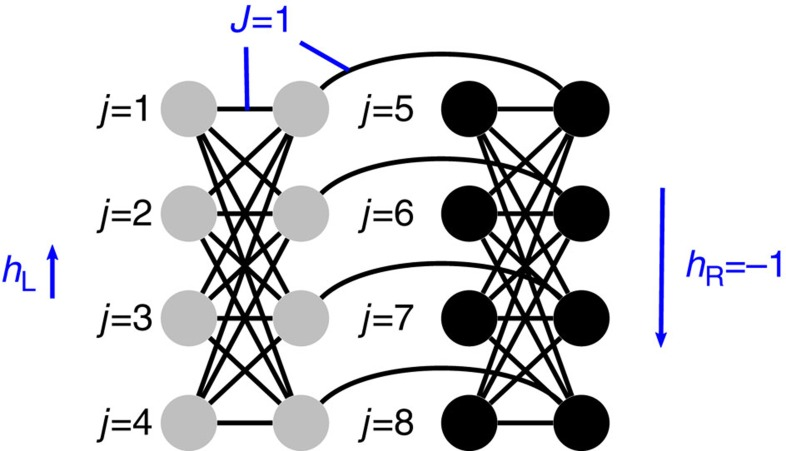
\includegraphics[height=1.75in]{chapters/Test-driving/tunnelling_probe}
\caption{The $16$-spin Ising Hamiltonian composed of two $K_{4,4}$ unit cells introduced in Ref.~\cite{Boixo:2014yu}. All couplings are set to $J=1$, all qubits in the left unit cell have a local field $0<h_L<0.5$ applied to them while all spins in the left unit cell have $h_R=1$ applied to them. Two local minima form, one with the cells internally aligned but in opposite states from each other (a local minimum) and the other with all states aligned with $h_R$ (the global minimum). By tightly binding each unit cell, they effectively act like single large spins.}
\label{fig:tunnelingprobe}
\end{figure}

Validating non-gate based quantum devices will continue to be a challenge as new such systems come online, but applying combinations of the techniques discussed above, from the construction of quantum signature Hamiltonians and tunneling probes to (in)direct proofs of entanglement via entanglement witnesses and direct computation of entanglement, should allow one to boost confidence that the system obeys the predictions of quantum theory \emph{over small scales}.
The challenge remains to extend these techniques so that they are able to demonstrate conclusively that a device with hundreds or thousands of qubits displays coherence and long-range entanglement.
Due to decoherence this presents a challenge for gate-based quantum devices as well even at a smaller scale \cite{PhysRevLett.106.130506,Bohnet:2016aa}, and speedup-inferred quantumness tests may prove to be simpler to execute than direct quantumness tests even in the gate-model setting.

\section{Benchmarking}
\label{section:benchmarking}

Assume we have at our disposal a device verified to be quantum, at least provisionally on the small scales covered by classical model rejection, and we would like to compare its performance to competing classical solvers. This is the task we refer to here as benchmarking, which belongs more generally to the field of experimental algorithmics \cite{McGeoch:book}. Specifically, consider the problem of estimating the value of some function of merit (or ``reward'') $R$ from the output of a given solver (e.g., our quantum device or some classical algorithm) for a given problem family $\mc{P} = \{P\}$. Each problem instance $P$ is parametrized by some parameters $\theta$. In the case of quantum annealers, particularly studies of the D-Wave devices thus far, the goal has generally been to find the ground state of Ising Hamiltonians as defined in Eq.~\eqref{eq:H}. In that context, typically the reward is taken to be the negative of the time to solution (TTS), defined as $\text{TTS}=t_f \log(1-p_d)/\log(1-p)$ for a probability $p$ of finding the ground state at least once with desired probability $p_d$ (typically $0.99$), and annealing time $t_f$.\footnote{The probability of not finding the ground state even once after $k$ independent runs of duration $t_f$ each is $(1-p)^k$, so the probability of finding it at least once is $1-(1-p)^k$, which we set equal to $p_d$. Solving for $k$ and substituting into $\text{TTS}=t_f k$ gives the TTS formula. See, e.g., Ref.~\cite{speedup} for a more detailed derivation.} In the language above, $R=-\text{TTS}$ (one would like to minimize the TTS), and the problem is parametrized by $\theta=\{h_i,J_{ij}\}$. Many similar metrics have been proposed, such as time-to-epsilon and time-to-target \cite{King:2015cs}, which amount to mild generalizations of TTS. A more elaborate notion of cost, based on optimal stopping theory, has also been considered and shown to recover the previous metrics as special cases \cite{Vinci:2016tg}. We shall return to this below.

\subsection{Prior work on benchmarking quantum annealers}

Our discussion here will focus exclusively on work that advanced the state of the art in benchmarking quantum annealers, and also primarily on those studies taken prior to or in the early phases of my PhD.

The first comprehensive study benchmarking QA devices was Ref.~\cite{q108}, using a $108$ qubit DW1 processor. This article introduced many of the concepts used in later studies in the field, including the above definition of the TTS. It focused on the performance on the set of random Ising problems with binary $\pm1$ local fields and couplings, and introduced the use of SA and SQA as important comparison algorithms. It also noted the importance of comparing against parallelized versions of classical algorithms, as quantum annealers such as the D-Wave device consume linearly more computational hardware with increasing problem size, and in many cases SA and SQA can be effectively parallelized in much the same way.

Another significant contribution of Ref.~\cite{q108} was the use of ``gauge averaging'' in benchmarking, a technique that was introduced in Ref.~\cite{q-sig} (where it was called ``spin inversions") and which has become so universal that it is now included natively in the D-Wave API for their processors, and which points toward a more general consideration for noisy quantum devices in the absence of quantum error correction.
The need for gauge averaging arises from the observation that in QA, one may have per-qubit or per-edge random and systematic biases from stray fields or interactions.
In such cases, performance may be dramatically impacted by the choice of mapping from a logical Hamiltonian as defined in Eq.~\eqref{eq:H} to a physically implemented computation.
In essence, a gauge transformation corresponds to swapping which physical spin state corresponds to a computational $0$ or $1$. In an ideal annealer, this transformation commutes with (i.e., is a symmetry of) the total Hamiltonian and so has no dynamical effect. However in the presence of noise, this symmetry is broken and the choice of gauge does make a difference, and indeed was found to have a significant effect on the performance of the DW1 quantum annealer, to such a degree that the device did not even correlate with itself if one compares one gauge to another, or even one gauge with itself when run later (most likely the result of slow drift $1/f$ noise resulting in the effect that each time the annealer is programmed, a small random error term is added to the Hamiltonian). However, when results for the same Hamiltonian were averaged across many gauges, the DW1 processor correlated quite well with itself \cite{q108}. Since then, applying many gauge transformations to the same Hamiltonian and averaging the results has become a standard practice in the QA community, and the idea behind it has been steadily generalized since then to include sampling over every known potentially broken symmetry of the Hamiltonian.

For example, if one is solving a fully connected Ising problem, the Hamiltonian has a permutation symmetry. Since every logical spin has an interaction with every other, one can relabel which spin is which without changing anything about the logical problem. However, when one goes to implement such a problem on an actual quantum annealer with limited connectivity, such as the DW2, one has to perform a minor embedding in which each logical spin is mapped to a chain of spins on the physical device \cite{Choi1,Choi2}. Those physical spins may have local field biases which vary from chain to chain, and thus the distribution over logical states will depend, in part, on the assignment of the logical spin variables to the physical chains, as shown in Ref.~\cite{Venturelli:2014nx}. This work was the first case study of both minor embedding of fully connected problems as well as permutation embeddings for such problems, and demonstrated the importance of optimizing the strength of the coupling in minor embedding applications, a topic which is discussed in more detail in Section~\ref{sec:err-corr}.

Finally, Ref.~\cite{MAX2SAT} demonstrated evidence for the easy-hard-easy phase transition for Max 2-SAT problems (wherein one wishes to find the maximal number of simultaneously satisfiable two-variable Boolean clauses over a set of variables from some ensemble of clauses) near a clause density of one, on the $108$-qubit DW1 processor. It performed a rudimentary benchmarking comparison between the DW1 and an exact Max 2-SAT solver (akmaxsat) (see also Ref.~\cite{McGeoch}), and noted that there was no correlation between the two solvers over randomly selected instances of Max 2-SAT. This work also introduced the important idea of bootstrapping into the QA community, variants of which (such as the Bayesian bootstrap \cite{rubin1981bayesian}) formed the backbone of error analyses for later studies, as a nonparametric method for approximating the distribution over the problem space and over the aforementioned broken computational symmetries, and will be discussed in much more detail in the next chapter, \ref{ch:benchmarking}.
